\documentclass{standalone}
\usepackage{tikz}
\usetikzlibrary{patterns, positioning}

\begin{document}
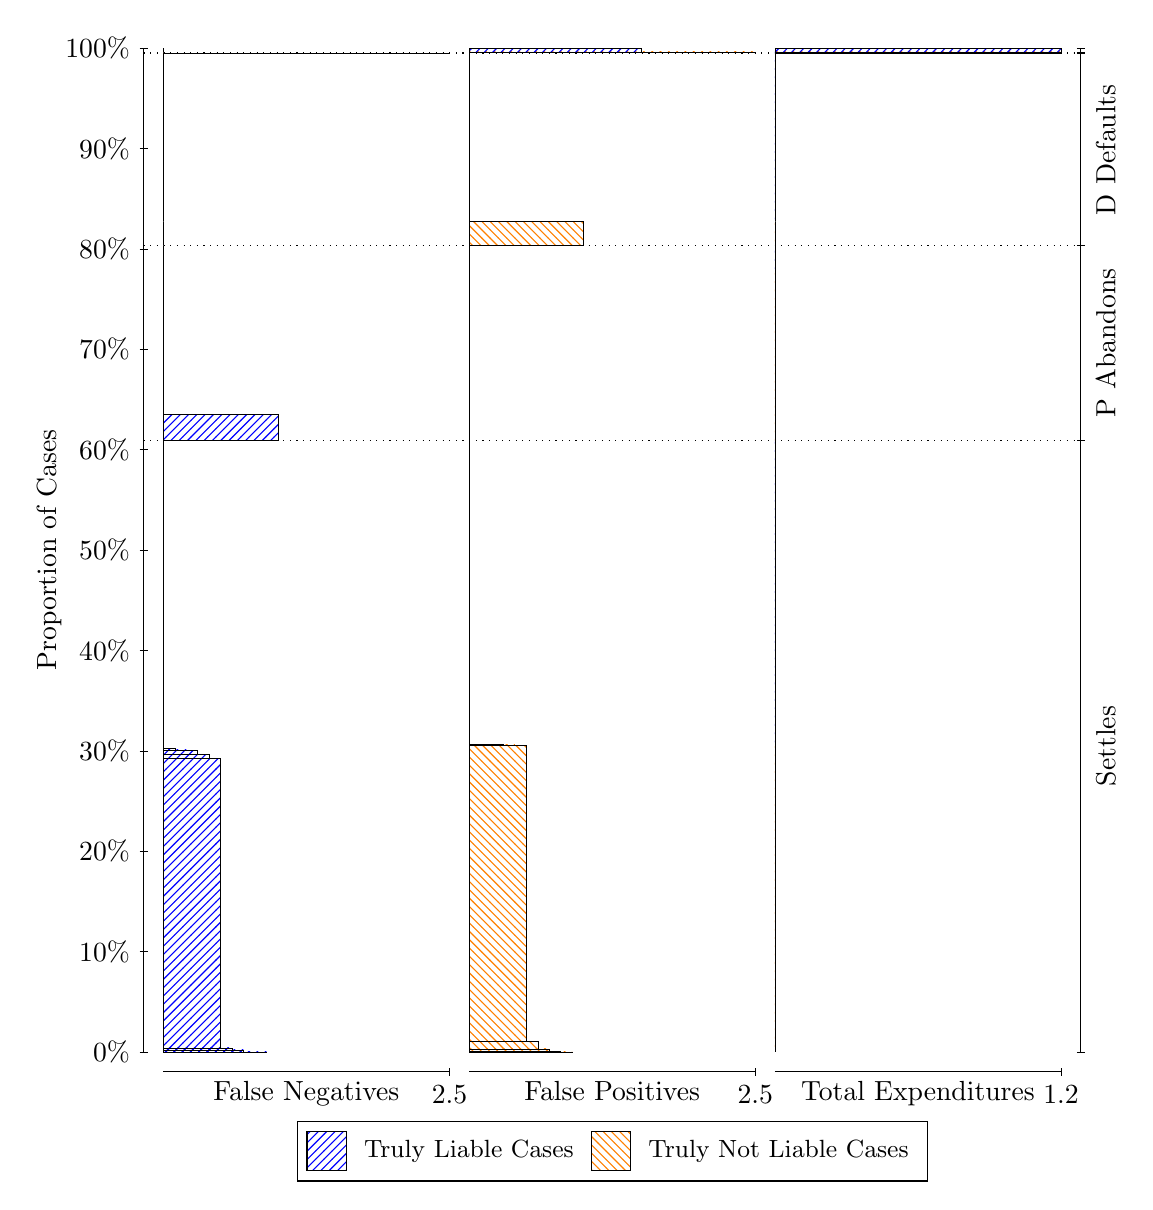
\begin{tikzpicture}
\draw[black, very thin] (1.5,1.75) -- (1.5,14.5);
\node[rotate=90, anchor=center] at (0.3, 8.125) {Proportion of Cases};
\draw[black, very thin] (1.45,1.75) -- (1.55,1.75);
\node[anchor=east] at (1.45, 1.75) {0\%};
\draw[black, very thin] (1.45,3.025) -- (1.55,3.025);
\node[anchor=east] at (1.45, 3.025) {10\%};
\draw[black, very thin] (1.45,4.3) -- (1.55,4.3);
\node[anchor=east] at (1.45, 4.3) {20\%};
\draw[black, very thin] (1.45,5.575) -- (1.55,5.575);
\node[anchor=east] at (1.45, 5.575) {30\%};
\draw[black, very thin] (1.45,6.85) -- (1.55,6.85);
\node[anchor=east] at (1.45, 6.85) {40\%};
\draw[black, very thin] (1.45,8.125) -- (1.55,8.125);
\node[anchor=east] at (1.45, 8.125) {50\%};
\draw[black, very thin] (1.45,9.4) -- (1.55,9.4);
\node[anchor=east] at (1.45, 9.4) {60\%};
\draw[black, very thin] (1.45,10.675) -- (1.55,10.675);
\node[anchor=east] at (1.45, 10.675) {70\%};
\draw[black, very thin] (1.45,11.95) -- (1.55,11.95);
\node[anchor=east] at (1.45, 11.95) {80\%};
\draw[black, very thin] (1.45,13.225) -- (1.55,13.225);
\node[anchor=east] at (1.45, 13.225) {90\%};
\draw[black, very thin] (1.45,14.5) -- (1.55,14.5);
\node[anchor=east] at (1.45, 14.5) {100\%};

\draw[black, very thin] (13.4,1.75) -- (13.4,14.5);
\draw[black, very thin] (13.35,1.75) -- (13.45,1.75);
\node[anchor=west] at (13.35, 1.75) {};
\draw[black, very thin] (13.35,9.5191) -- (13.45,9.5191);
\node[anchor=west] at (13.35, 9.5191) {};
\draw[black, very thin] (13.35,11.989) -- (13.45,11.989);
\node[anchor=west] at (13.35, 11.989) {};
\draw[black, very thin] (13.35,14.427) -- (13.45,14.427);
\node[anchor=west] at (13.35, 14.427) {};
\draw[black, very thin] (13.35,14.443) -- (13.45,14.443);
\node[anchor=west] at (13.35, 14.443) {};
\draw[black, very thin] (13.35,14.5) -- (13.45,14.5);
\node[anchor=west] at (13.35, 14.5) {};

\draw[black, very thin, pattern color=blue, pattern=north east lines] (1.75,1.75) rectangle (3.058,1.7506);
\draw[black, very thin, pattern color=blue, pattern=north east lines] (1.75,1.7506) rectangle (2.9127,1.751);
\draw[black, very thin, pattern color=blue, pattern=north east lines] (1.75,1.751) rectangle (2.7673,1.776);
\draw[black, very thin, pattern color=blue, pattern=north east lines] (1.75,1.776) rectangle (2.622,1.7763);
\draw[black, very thin, pattern color=blue, pattern=north east lines] (1.75,1.7763) rectangle (2.622,1.8011);
\draw[black, very thin, pattern color=blue, pattern=north east lines] (1.75,1.8011) rectangle (2.4767,5.4768);
\draw[black, very thin, pattern color=blue, pattern=north east lines] (1.75,5.4768) rectangle (2.3313,5.5338);
\draw[black, very thin, pattern color=blue, pattern=north east lines] (1.75,5.5338) rectangle (2.186,5.582);
\draw[black, very thin, pattern color=blue, pattern=north east lines] (1.75,5.582) rectangle (2.0407,5.5866);
\draw[black, very thin, pattern color=blue, pattern=north east lines] (1.75,5.5866) rectangle (1.8953,5.6095);
\draw[black, very thin, pattern color=orange, pattern=north west lines] (1.75,5.6095) rectangle (1.75,9.5191);
\draw[black, very thin, pattern color=blue, pattern=north east lines] (1.75,9.5191) rectangle (3.2033,9.851);
\draw[black, very thin, pattern color=orange, pattern=north west lines] (1.75,9.851) rectangle (1.75,11.989);
\draw[black, very thin, pattern color=orange, pattern=north west lines] (1.75,11.989) rectangle (1.75,12.3);
\draw[black, very thin, pattern color=blue, pattern=north east lines] (1.75,12.3) rectangle (1.75,14.427);
\draw[black, very thin, pattern color=blue, pattern=north east lines] (1.75,14.427) rectangle (5.3833,14.434);
\draw[black, very thin, pattern color=orange, pattern=north west lines] (1.75,14.434) rectangle (1.75,14.443);
\draw[black, very thin, pattern color=orange, pattern=north west lines] (1.75,14.443) rectangle (1.75,14.451);
\draw[black, very thin, pattern color=blue, pattern=north east lines] (1.75,14.451) rectangle (1.75,14.5);
\draw[black, very thin, pattern color=orange, pattern=north west lines] (5.6333,1.75) rectangle (6.9413,1.7525);
\draw[black, very thin, pattern color=orange, pattern=north west lines] (5.6333,1.7525) rectangle (6.796,1.7537);
\draw[black, very thin, pattern color=orange, pattern=north west lines] (5.6333,1.7537) rectangle (6.6507,1.7899);
\draw[black, very thin, pattern color=orange, pattern=north west lines] (5.6333,1.7899) rectangle (6.5053,1.8831);
\draw[black, very thin, pattern color=orange, pattern=north west lines] (5.6333,1.8831) rectangle (6.36,5.6426);
\draw[black, very thin, pattern color=orange, pattern=north west lines] (5.6333,5.6426) rectangle (6.2147,5.6502);
\draw[black, very thin, pattern color=orange, pattern=north west lines] (5.6333,5.6502) rectangle (6.2147,5.6504);
\draw[black, very thin, pattern color=orange, pattern=north west lines] (5.6333,5.6504) rectangle (6.0693,5.6583);
\draw[black, very thin, pattern color=orange, pattern=north west lines] (5.6333,5.6583) rectangle (5.924,5.6585);
\draw[black, very thin, pattern color=orange, pattern=north west lines] (5.6333,5.6585) rectangle (5.7787,5.6595);
\draw[black, very thin, pattern color=blue, pattern=north east lines] (5.6333,5.6595) rectangle (5.6333,9.5191);
\draw[black, very thin, pattern color=orange, pattern=north west lines] (5.6333,9.5191) rectangle (5.6333,11.657);
\draw[black, very thin, pattern color=blue, pattern=north east lines] (5.6333,11.657) rectangle (5.6333,11.989);
\draw[black, very thin, pattern color=orange, pattern=north west lines] (5.6333,11.989) rectangle (7.0867,12.3);
\draw[black, very thin, pattern color=blue, pattern=north east lines] (5.6333,12.3) rectangle (5.6333,14.427);
\draw[black, very thin, pattern color=orange, pattern=north west lines] (5.6333,14.427) rectangle (5.6333,14.436);
\draw[black, very thin, pattern color=blue, pattern=north east lines] (5.6333,14.436) rectangle (5.6333,14.443);
\draw[black, very thin, pattern color=orange, pattern=north west lines] (5.6333,14.443) rectangle (9.2667,14.451);
\draw[black, very thin, pattern color=blue, pattern=north east lines] (5.6333,14.451) rectangle (7.8133,14.5);
\draw[black, very thin, pattern color=orange, pattern=north west lines] (9.5167,1.75) rectangle (9.5167,5.6595);
\draw[black, very thin, pattern color=blue, pattern=north east lines] (9.5167,5.6595) rectangle (9.5167,9.5191);
\draw[black, very thin, pattern color=orange, pattern=north west lines] (9.5167,9.5191) rectangle (9.5167,11.657);
\draw[black, very thin, pattern color=blue, pattern=north east lines] (9.5167,11.657) rectangle (9.5167,11.989);
\draw[black, very thin, pattern color=orange, pattern=north west lines] (9.5167,11.989) rectangle (9.5167,12.3);
\draw[black, very thin, pattern color=blue, pattern=north east lines] (9.5167,12.3) rectangle (9.5167,14.427);
\draw[black, very thin, pattern color=orange, pattern=north west lines] (9.5167,14.427) rectangle (13.15,14.436);
\draw[black, very thin, pattern color=blue, pattern=north east lines] (9.5167,14.436) rectangle (13.15,14.443);
\draw[black, very thin, pattern color=orange, pattern=north west lines] (9.5167,14.443) rectangle (13.15,14.451);
\draw[black, very thin, pattern color=blue, pattern=north east lines] (9.5167,14.451) rectangle (13.15,14.5);
\draw[black, dotted] (1.5,9.5191) -- (13.4,9.5191);
\draw[black, dotted] (1.5,11.989) -- (13.4,11.989);
\draw[black, dotted] (1.5,14.427) -- (13.4,14.427);
\draw[black, dotted] (1.5,14.443) -- (13.4,14.443);
\draw[black, very thin] (1.75,1.5) -- (5.3833,1.5);
\node[anchor=north] at (3.5667, 1.5) {False Negatives};
\draw[black, very thin] (5.3833,1.45) -- (5.3833,1.55);
\node[anchor=north] at (5.3833, 1.45) {2.5};

\draw[black, very thin] (5.6333,1.5) -- (9.2667,1.5);
\node[anchor=north] at (7.45, 1.5) {False Positives};
\draw[black, very thin] (9.2667,1.45) -- (9.2667,1.55);
\node[anchor=north] at (9.2667, 1.45) {2.5};

\draw[black, very thin] (9.5167,1.5) -- (13.15,1.5);
\node[anchor=north] at (11.333, 1.5) {Total Expenditures};
\draw[black, very thin] (13.15,1.45) -- (13.15,1.55);
\node[anchor=north] at (13.15, 1.45) {1.2};

\node[black, centered, rotate=90] at (13.72, 5.6345) {Settles};
\node[black, centered, rotate=90] at (13.72, 10.754) {P Abandons};
\node[black, centered, rotate=90] at (13.72, 13.208) {D Defaults};



\draw (7.449999999999999,1.5) node[draw=none] (baseCoordinate) {};
\begin{scope}[align=center]
        \matrix[scale=0.5, draw=black, below=0.5cm of baseCoordinate, nodes={draw}, column sep=0.1cm]{
            \node[rectangle, draw, minimum width=0.5cm, minimum height=0.5cm, pattern=north east lines, pattern color=blue] {}; &
            \node[draw=none, font=\small] (B) {Truly Liable Cases}; &
            \node[rectangle, draw, minimum width=0.5cm, minimum height=0.5cm, pattern=north west lines, pattern color=orange] {}; &
            \node[draw=none, font=\small] (B) {Truly Not Liable Cases}; \\
            };
\end{scope}

\end{tikzpicture}
\end{document}